\documentclass[11pt]{amsart}
\usepackage[a4paper,bindingoffset=0.2in,left=1in,right=1in,top=1in,bottom=1in,footskip=.25in]{geometry}
\geometry{letterpaper}                   % ... or a4paper or a5paper or ... 
%\geometry{landscape}                % Activate for for rotated page geometry
%\usepackage[parfill]{parskip}    % Activate to begin paragraphs with an empty line rather than an indent
\usepackage{graphicx}
\usepackage{amssymb}
\usepackage{epstopdf}
\usepackage{tikz}
\usepackage{ wasysym }
\usepackage{lineno}
\usepackage{graphicx}
\setlength\parindent{0pt}
\DeclareGraphicsRule{.tif}{png}{.png}{`convert #1 `dirname #1`/`basename #1 .tif`.png}
\renewcommand{\thesubsection}{\arabic{subsection}}

\title{PS1}
\author{Stefan Peterson}
\date{}                                           % Activate to display a given date or no date

\begin{document}
\raggedright
\maketitle	

\begingroup
\Huge\section{Short answer problems}
\endgroup

\subsection{}
\textbf{Give an example of how one can exploit the associative property of convolution to more efficiently filter an image.} \\
\vspace{5mm}
Convolution generally requires smoothing via a Gaussian filter first but instead of applying that filter and then applying the derivative, since convolution is associative we can apply the derivative to the Gaussian filter and then apply that resulting filter to the image.

\subsection{}
\textbf{This is the input image: [0 0 1 1 0 0 1 1]. What is the result of dilation with a structuring element[1 1 1]?} \\
\vspace{5mm}
\begin{center}
[0 1 1 1 1 1 1 1]
\end{center}

\subsection{}
\textbf{The filter f' = [0 -1/2 0 1/2 0] gives an estimate of the first derivative of the image in the x direction. What is the corresponding second derivative filter f''? (Hint: Asymmetric filters must be flipped prior to convolution.)} \\
\vspace{5mm}
\begin{center}
[$\frac{1}{4}$ 0 $\frac{-1}{2}$ 0 $\frac{1}{4}$] \\
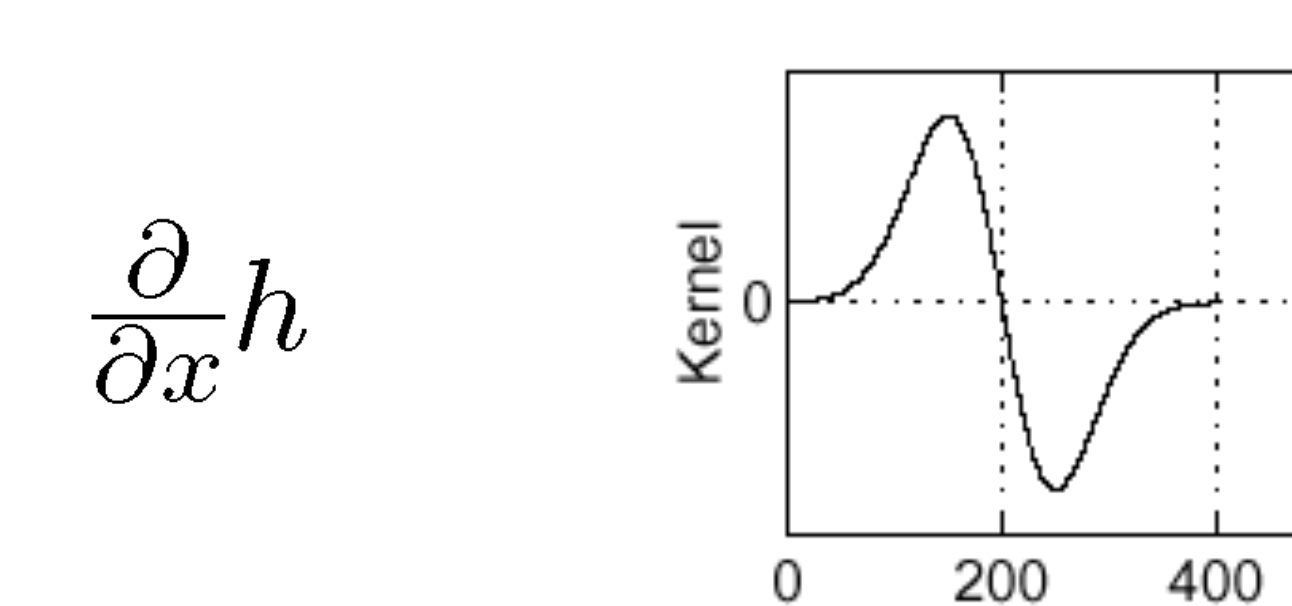
\includegraphics[scale=0.25]{derivative.png}
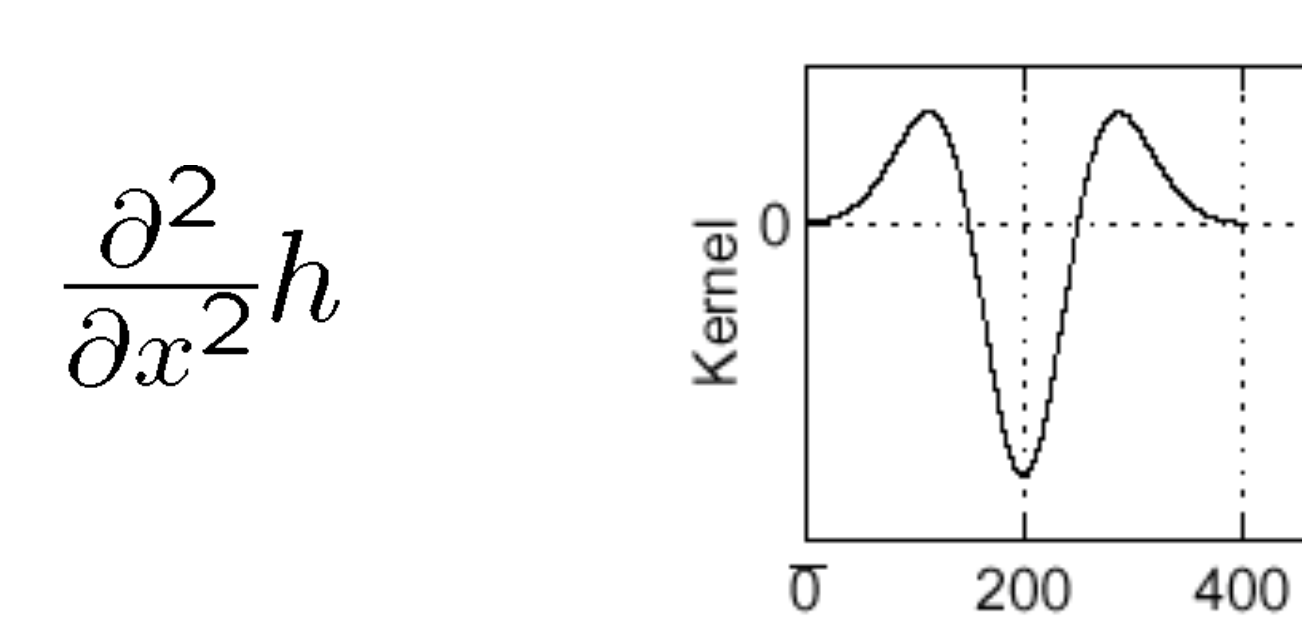
\includegraphics[scale=0.25]{second-derivative.png}
\end{center}


\subsection{}
\textbf{Describe a possible flaw in the use of additive Gaussian noise to represent image noise.}\\
\vspace{5mm}

\subsection{}
\textbf{Design a method that takes video data from a camera perched above a conveyor belt at an automotive equipment manufacturer, and reports any flaws in the assembly of a part. Your response should be a list of concise, specific steps, and should incorporate several techniques covered in class thus far. Specify any important assumptions your method makes.} \\
\vspace{5mm}
We will assume the following:
\begin{itemize}
\item Constant lighting in the area
\item The parts will always have the same orientation and location on the belt
\item The parts are evenly spaced on the belt
\item The program has an image with which to compare that is known to be flawless which we will call the Golden Master (GM)
\end{itemize}

Then we can do:
\begin{enumerate}
\item Take the image at the predetermined location on the belt
\item Texture analysis:
	\begin{enumerate}
	\item Apply each filter in given filter bank to image
	\item Classify regions based on mean absolute response
	\item Use this to compare to GM
	\end{enumerate}
\item Edge analysis:
	\begin{enumerate}
	\item Filter image with derivative of Gaussian
	\item Find magnitude and orientation of gradient
	\item Apply hysteresis thresholding (use high threshold to start edge curves and low to continue them)
	\item Use chamfer distance to compare current image to GM
	\end{enumerate}
\item Binary image analysis:
	\begin{enumerate}
	\item Convert image to binary form
	\item Using morphological operators, clean up the thresholded image
	\item Find connected components
	\item Use connected components to compare current image to GM
	\end{enumerate}
\end{enumerate}







\begingroup
\Huge\section{Programming problem: content-aware image resizing}
\endgroup

\subsection{}
\textbf{Reduce width by 100:} \\
\begin{center}
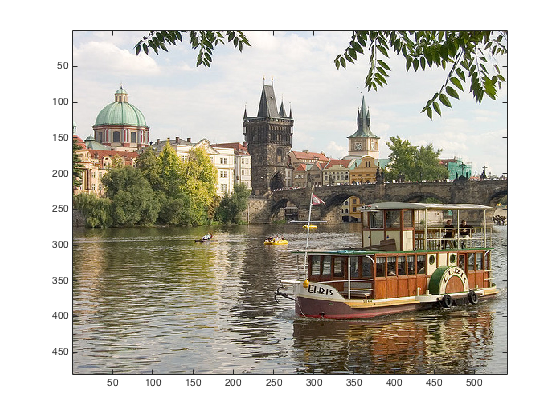
\includegraphics[scale=0.40]{outputReduceWidthPrague.png}
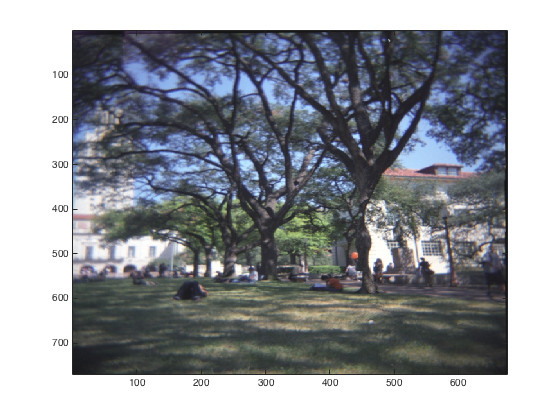
\includegraphics[scale=0.40]{outputReduceWidthMall.png}
\end{center}

\subsection{}
\textbf{Reduce height by 100:} \\
\begin{center}
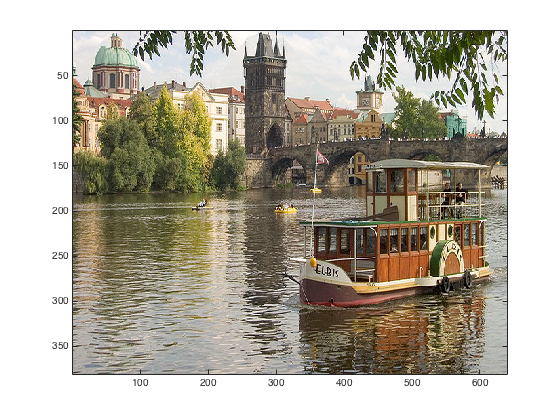
\includegraphics[scale=0.40]{outputReduceHeightPrague.png}
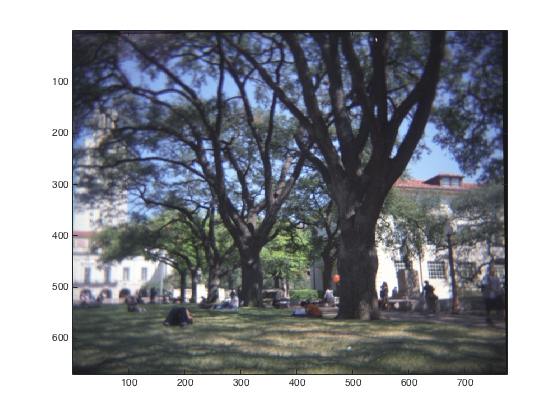
\includegraphics[scale=0.40]{outputReduceHeightMall.png}
\end{center}

\subsection{}
\textbf{Energy map and vertical/horizontal minimum energy maps:} \\
\begin{center}
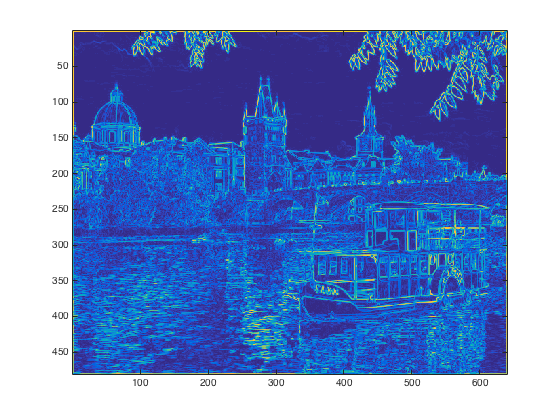
\includegraphics[scale=0.60]{energyMapPrague.png}
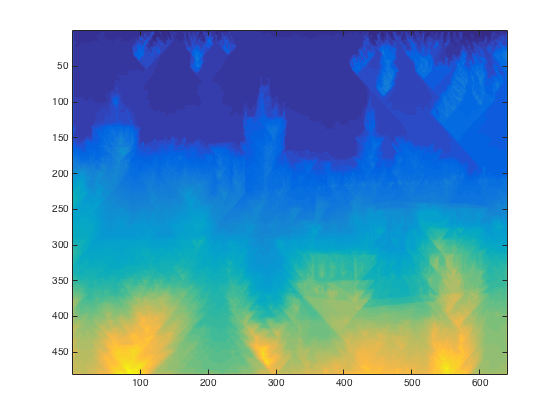
\includegraphics[scale=0.40]{energyMapVerticalPrague.png}
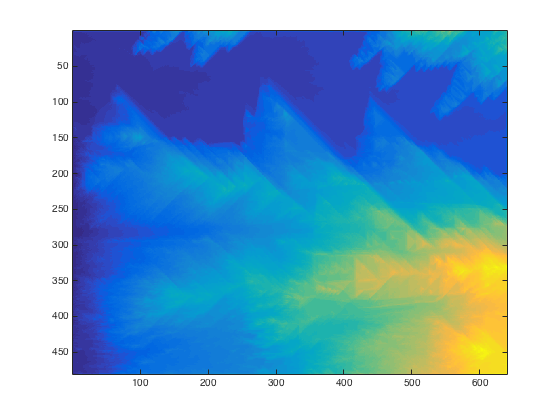
\includegraphics[scale=0.40]{energyMapHorizontalPrague.png}
The vertical energy map displayed on the left starts at the top of the image and goes downwards choosing values based the minimum total energy path across the image, subject to eight connectedness. \\

The horizontal energy map displayed on the right starts at the left of the image and goes right choosing values based the minimum total energy path across the image, subject to eight connectedness. \\

\end{center}

\subsection{}
\textbf{Vertical and horizontal seams} \\
\begin{center}
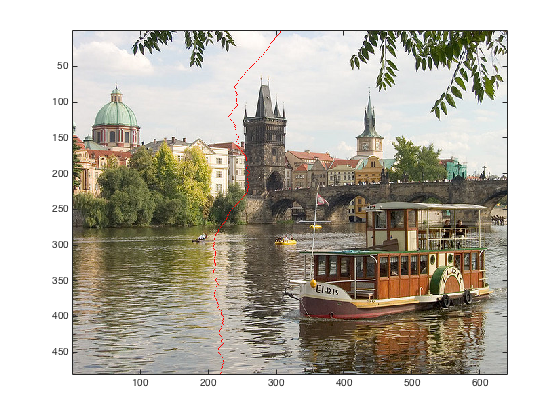
\includegraphics[scale=0.40]{verticalSeamPrague.png}
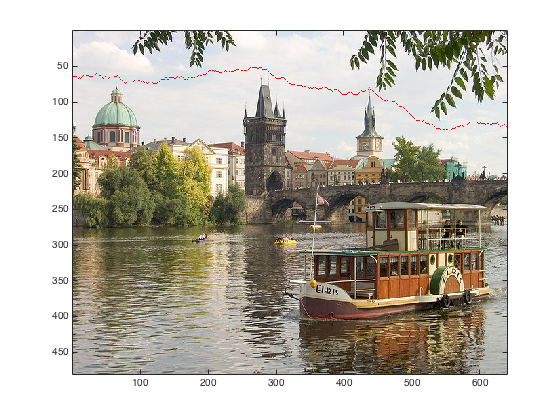
\includegraphics[scale=0.40]{horizontalSeamPrague.png}
\end{center}

\subsection{}
\textbf{Different filter for energy function computation} \\
\begin{center}

\end{center}

\subsection{}
\textbf{Custom images and resizing} \\
\begin{center}
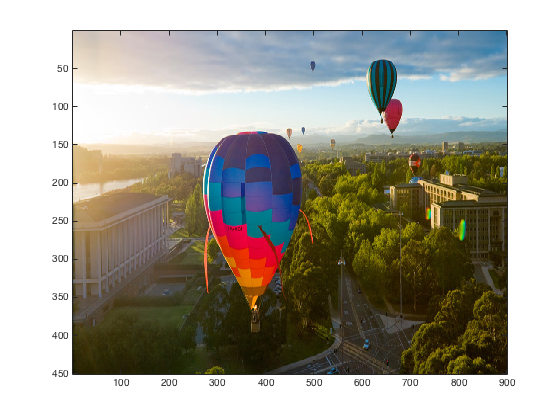
\includegraphics[scale=0.40]{originalBallons.png}
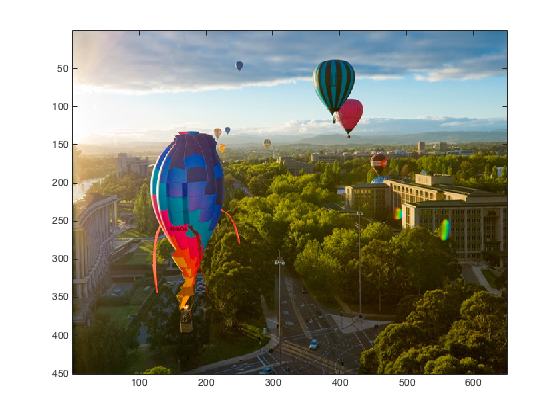
\includegraphics[scale=0.40]{outputReduceWidthBalloons.png}
Reducing the width for some reason destroys what we perceive to be the center of focus in the image but this is likely due to the fact that the vast majority of the colors in that object are bright and relatively close in color, and as they do change, they change in a gradient going from dark to light as they move downward. \\
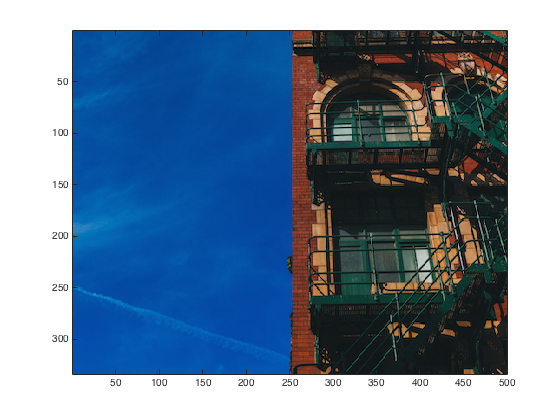
\includegraphics[scale=0.40]{originalStairs.png}
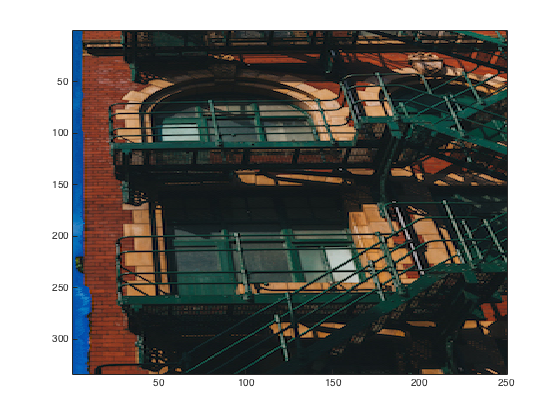
\includegraphics[scale=0.40]{outputReduceWidthStairs.png}
Reducing the width deletes the "unimportant" sky landscape almost entirely before altering the "important" building. \\
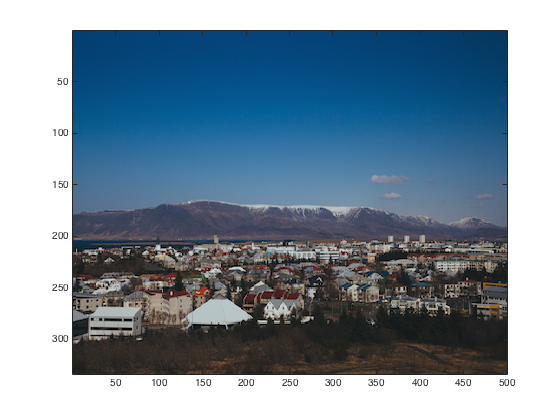
\includegraphics[scale=0.40]{originalVillage.png}
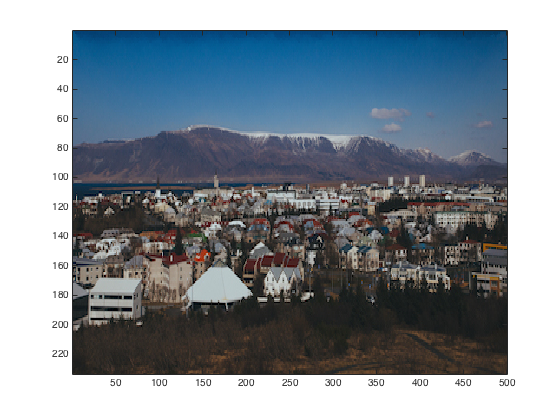
\includegraphics[scale=0.40]{outputReduceHeightVillage.png}
Similarly, reducing the height deletes the "unimportant" sky landscape almost entirely before altering the "important" village below. \\

\end{center}




\begingroup
\Huge\section{Extra credit}
\endgroup



\end{document}  